\documentclass{ctexart}
\textheight 23.5cm \textwidth 15.8cm
\topmargin -1.5cm \oddsidemargin 0.3cm \evensidemargin -0.3cm

\usepackage{verbatim}
\usepackage{amsmath}
\usepackage{amssymb}
\usepackage{fancyhdr}
\usepackage{graphicx}
\usepackage{listings}
\usepackage[table]{xcolor}

\title{DDPM 从入门到入土}
\author{郭东昊 \quad 高歌}

\begin{document}
\maketitle

\section{引言 (Introduction)}

\noindent
近年来,生成模型(Generative Models)在机器学习领域取得了突破性进展,其在图像生成、风格迁移、数据增强等任务中展现了惊人的能力。在众多生成模型中,去噪扩散概率模型(Denoising Diffusion Probabilistic Models, DDPM)作为一种新兴且强大的模型,受到了广泛关注。

\noindent
DDPM 的核心思想源于对非平衡热力学的观察。它包含两个关键过程:
\begin{enumerate}
    \item \textbf{前向过程(Forward Process)}:也称为扩散过程(Diffusion Process)。在这个过程中,模型通过数千个时间步(steps),逐渐地向原始数据(如一张清晰的图片)中添加微量的高斯噪声。随着时间的推移,原始数据最终会变成一个完全无规律的、符合标准正态分布的噪声图像。这个过程是固定的,不涉及任何模型学习。
    \item \textbf{逆向过程(Reverse Process)}:这是模型的核心学习部分。模型学习如何系统地“撤销”前向过程中添加的噪声。从一个纯粹的噪声图像开始,模型利用一个深度神经网络(通常是 U-Net 架构)在每个时间步预测并去除一小部分噪声,逐步将噪声图像还原成一张清晰、真实的图像。
\end{enumerate}
通过学习这个逆向的去噪过程,DDPM 能够从随机噪声中生成高质量、高保真的数据样本。本报告将详细阐述 DDPM 的数学原理,并介绍其依赖的相关技术。

\section{相关工作 (Related Work)}

\subsection{U-Net 架构}
\noindent
U-Net 是一种最初为生物医学图像分割而设计的卷积神经网络架构,但由于其出色的性能,现已广泛应用于各种图像到图像(Image-to-Image)的转换任务中,包括 DDPM 中的噪声预测。

\noindent
U-Net 的结构呈 “U” 形,由两个主要部分组成:
\begin{itemize}
    \item \textbf{收缩路径(Contracting Path)}:也被称为编码器(Encoder)。它由一系列标准的卷积层和最大池化层(Max Pooling)组成。在收缩路径中,输入图像的空间维度(高度和宽度)被逐渐减小,而特征图的通道数(深度)则相应增加。这个过程旨在捕捉图像的上下文信息和高级特征。
    \item \textbf{扩张路径(Expansive Path)}:也被称为解码器(Decoder)。它通过上采样(Up-sampling)或转置卷积(Transposed Convolution)将特征图的空间维度逐步恢复到原始输入图像的大小。扩张路径的关键创新在于 \textbf{跳跃连接(Skip Connections)}。这些连接将收缩路径中对应层级的特征图直接拼接到扩张路径的相应层级上。这一操作使得解码器在恢复空间细节时,能够直接利用编码器捕捉到的低级、高分辨率的特征,从而极大地提高了定位精度和细节还原能力。
\end{itemize}

\noindent 
在DDPM 中,U-Net 的任务是在给定当前时间步 $t$ 的噪声图像 $x_t$ 的情况下,预测出该图像中包含的噪声 $\epsilon$。U-Net 的输入是噪声图像 $x_t$ 和当前时间步 $t$ 的嵌入表示,输出是一个与输入图像尺寸完全相同的噪声预测图。其强大的特征融合能力使其能够精确地预测噪声,从而在逆向过程中逐步恢复出清晰图像。

 \begin{figure}[htb]
     \centering
     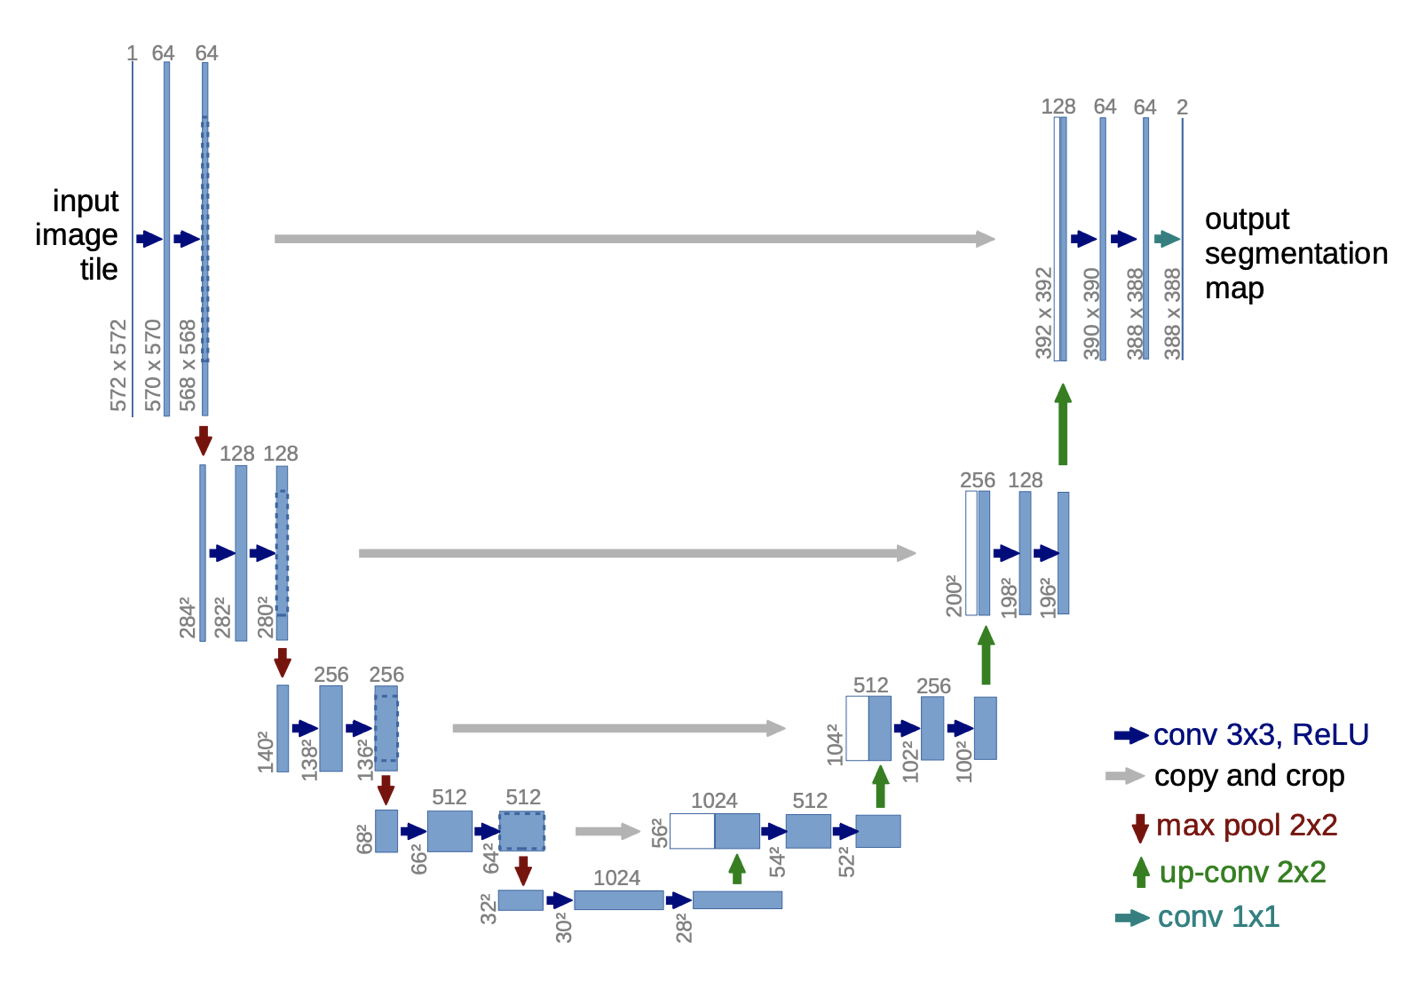
\includegraphics[width=0.8\textwidth]{unet.png}
     \caption{U-Net}
     \label{fig:unet}
 \end{figure}

\subsection{ReLU 激活函数}
\noindent
修正线性单元(Rectified Linear Unit, ReLU)是深度学习中最常用的激活函数之一。它的数学定义非常简单:
$$ f(x) = \max(0, x) $$
ReLU 的主要优点在于:
\begin{itemize}
    \item \textbf{解决梯度消失问题}:对于正输入,ReLU 的导数为 1,这有助于在深层网络中维持梯度的流动,避免了 Sigmoid 和 Tanh 等函数在饱和区(输入值过大或过小)梯度接近于零的问题。
    \item \textbf{计算效率高}:ReLU 的计算只涉及一个简单的阈值操作,比 Sigmoid 和 Tanh 等函数中的指数运算要快得多。
    \item \textbf{引入稀疏性}:当输入为负时,ReLU 的输出为零,这可以使网络中的一部分神经元处于非激活状态,从而引入稀疏性,有助于模型更好地提取特征。
\end{itemize}

\subsection{变分自编码器 (Variational Autoencoder, VAE)}
\noindent
变分自编码器(VAE)是一种重要的生成模型,其核心思想与 DDPM 的损失函数推导密切相关。VAE 同样由编码器和解码器组成,但它引入了概率论的视角。
\begin{itemize}
    \item \textbf{编码器} $Q(z|X)$:将输入数据 $X$ 编码为一个概率分布,通常是高斯分布 $\mathcal{N}(\mu, \Sigma)$,而不是一个固定的向量。
    \item \textbf{解码器} $P(X|z)$:从编码器产生的分布中采样一个隐变量 $z$,然后解码器学习从 $z$ 重建原始数据 $X$。
\end{itemize}
\noindent
VAE 的训练目标是最大化证据下界(Evidence Lower Bound, ELBO),也称为变分下界(Variational Lower Bound, VLB)。ELBO 由两部分组成:
$$ \mathcal{L}_{\text{ELBO}} = \mathbb{E}_{z \sim Q(z|X)}[\log P(X|z)] - D_{KL}(Q(z|X) || P(z)) $$
其中,第一项是 \textbf{重建损失},鼓励解码器精确地重建输入数据。第二项是 \textbf{KL 散度},作为一个正则化项,它衡量编码器输出的分布 $Q(z|X)$ 与一个预设的先验分布 $P(z)$(通常是标准正态分布 $\mathcal{N}(0, I)$)之间的相似性。这个正则化项使得隐空间(latent space)变得平滑和连续,从而让模型具备从隐空间中随机采样并生成新数据的能力。DDPM 的损失函数正是基于最大化对数似然的变分下界这一思想推导出来的。

\section{DDPM 核心原理}

\subsection{前向过程 (Forward Process)}
\noindent
前向过程是一个固定的、不可学习的马尔可夫链,它逐步向原始数据 $x_0$ 中添加高斯噪声。假设整个过程有 $T$ 个时间步,在每个时间步 $t$,我们向 $x_{t-1}$ 中加入一个方差为 $\beta_t$ 的高斯噪声,得到 $x_t$。这个单步转移可以表示为:
$$ q(x_t | x_{t-1}) = \mathcal{N}(x_t; \sqrt{1 - \beta_t} x_{t-1}, \beta_t I) $$
其中,$\{\beta_t\}_{t=1}^T$ 是一个预先设定的方差表(variance schedule),通常是从一个较小的值(如 $10^{-4}$)线性增加到一个较大的值(如 $0.02$)。令 $\alpha_t = 1 - \beta_t$ 和 $\bar{\alpha}_t = \prod_{i=1}^{t} \alpha_i$,通过重参数化技巧(reparameterization trick),我们可以推导出 $x_t$ 与 $x_0$ 之间的直接关系:
\begin{align*}
    x_t &= \sqrt{\alpha_t}x_{t-1} + \sqrt{1-\alpha_t}\epsilon_{t-1} \\
    &= \sqrt{\alpha_t}(\sqrt{\alpha_{t-1}}x_{t-2} + \sqrt{1-\alpha_{t-1}}\epsilon_{t-2}) + \sqrt{1-\alpha_t}\epsilon_{t-1} \\
    &= \sqrt{\alpha_t\alpha_{t-1}}x_{t-2} + \sqrt{\alpha_t(1-\alpha_{t-1})}\epsilon_{t-2} + \sqrt{1-\alpha_t}\epsilon_{t-1} \\
    &= \dots \\
    &= \sqrt{\bar{\alpha}_t}x_0 + \sqrt{1 - \bar{\alpha}_t}\epsilon
\end{align*}
其中 $\epsilon \sim \mathcal{N}(0, I)$。这个性质非常重要,它意味着我们可以在任意时间步 $t$ 直接从原始数据 $x_0$ 采样得到 $x_t$,而无需迭代计算。因此,从 $x_0$ 到 $x_t$ 的采样分布为:
$$ q(x_t | x_0) = \mathcal{N}(x_t; \sqrt{\bar{\alpha}_t} x_0, (1 - \bar{\alpha}_t) I) $$

 \begin{figure}[htb]
    \centering
    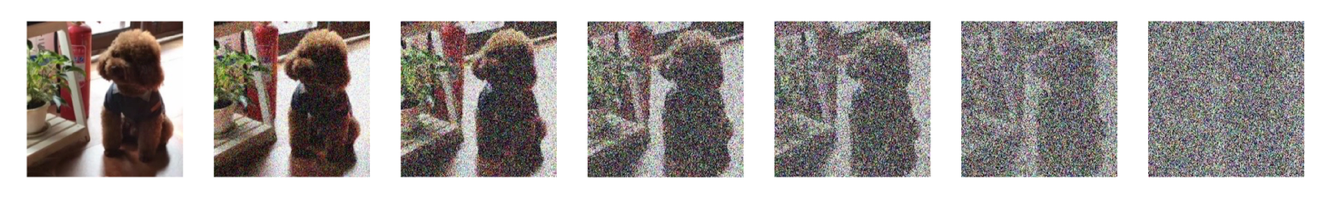
\includegraphics[width=0.9\textwidth]{forward.png}
    \caption{forward process}
    \label{fig:forward}
 \end{figure}

\subsection{逆向过程 (Reverse Process)}
\noindent
逆向过程是 DDPM 的核心学习任务,其目标是学习一个模型来逆转上述加噪过程,即从一个纯噪声 $x_T \sim \mathcal{N}(0, I)$ 出发,逐步去除噪声,最终恢复出原始数据 $x_0$。这个过程也是一个马尔可夫链,由一个神经网络 $p_\theta$ 参数化:
$$ p_\theta(x_{0:T}) = p(x_T) \prod_{t=1}^T p_\theta(x_{t-1} | x_t) $$
其中 $p_\theta(x_{t-1} | x_t)$ 表示在给定 $x_t$ 的情况下,模型预测的 $x_{t-1}$ 的分布。我们将其建模为高斯分布:
$$ p_\theta(x_{t-1} | x_t) = \mathcal{N}(x_{t-1}; \mu_\theta(x_t, t), \Sigma_\theta(x_t, t)) $$

\noindent
为了训练这个逆向过程,我们需要知道 $x_{t-1}$ 的真实后验分布。利用贝叶斯定理,我们可以推导出给定 $x_t$ 和 $x_0$ 时 $x_{t-1}$ 的后验分布:
$$ q(x_{t-1} | x_t, x_0) = \frac{q(x_t | x_{t-1}, x_0) q(x_{t-1} | x_0)}{q(x_t | x_0)} $$

\noindent
由于前向过程是马尔可夫链,$q(x_t | x_{t-1}, x_0) = q(x_t | x_{t-1})$,因此:
$$ q(x_{t-1} | x_t, x_0) = \frac{q(x_t | x_{t-1}) q(x_{t-1} | x_0)}{q(x_t | x_0)} $$

\noindent
前向过程中的各个条件概率都是高斯分布,因此这个后验分布也是高斯分布:
$$ q(x_{t-1} | x_t, x_0) = \mathcal{N}(x_{t-1}; \tilde{\mu}_t(x_t, x_0), \tilde{\beta}_t I) $$

\noindent
对高斯分布进行代数运算后,我们可以得到这个后验分布的均值和方差:
$$ \tilde{\mu}_t(x_t, x_0) = \frac{\sqrt{\bar{\alpha}_{t-1}}\beta_t}{1-\bar{\alpha}_t}x_0 + \frac{\sqrt{\alpha_t}(1-\bar{\alpha}_{t-1})}{1-\bar{\alpha}_t}x_t $$
$$ \tilde{\beta}_t = \frac{1-\bar{\alpha}_{t-1}}{1-\bar{\alpha}_t}\beta_t $$

\noindent
然而,在实际的逆向过程中,我们无法获取真实的 $x_0$。我们可以利用前向过程的性质,从 $x_t$ 反解出 $x_0$ 的估计值。回顾前向过程的公式:
$$ x_t = \sqrt{\bar{\alpha}_t}x_0 + \sqrt{1 - \bar{\alpha}_t}\epsilon $$

\noindent
重新整理,我们可以表示 $x_0$ 为:
$$ x_0 = \frac{1}{\sqrt{\bar{\alpha}_t}}(x_t - \sqrt{1-\bar{\alpha}_t}\epsilon) $$

\noindent
因此,如果我们能预测在时间步 $t$ 添加的噪声 $\epsilon$,我们就能估计 $x_0$。这就是为什么我们训练一个神经网络 $\epsilon_\theta(x_t, t)$ 来预测噪声。将 $x_0$ 的估计值代入 $\tilde{\mu}_t$ 的公式中,我们得到:

\begin{align*}
\tilde{\mu}_t(x_t, x_0) &= \frac{\sqrt{\bar{\alpha}_{t-1}}\beta_t}{1-\bar{\alpha}_t} \cdot \frac{1}{\sqrt{\bar{\alpha}_t}}(x_t - \sqrt{1-\bar{\alpha}_t}\epsilon_\theta) + \frac{\sqrt{\alpha_t}(1-\bar{\alpha}_{t-1})}{1-\bar{\alpha}_t}x_t \\
&= \frac{\sqrt{\bar{\alpha}_{t-1}}\beta_t}{\sqrt{\bar{\alpha}_t}(1-\bar{\alpha}_t)}x_t - \frac{\sqrt{\bar{\alpha}_{t-1}}\beta_t\sqrt{1-\bar{\alpha}_t}}{\sqrt{\bar{\alpha}_t}(1-\bar{\alpha}_t)}\epsilon_\theta + \frac{\sqrt{\alpha_t}(1-\bar{\alpha}_{t-1})}{1-\bar{\alpha}_t}x_t
\end{align*}

\noindent
经过代数简化,我们可以得到模型预测的均值 $\mu_\theta$:
$$ \mu_\theta(x_t, t) = \frac{1}{\sqrt{\alpha_t}}\left(x_t - \frac{\beta_t}{\sqrt{1-\bar{\alpha}_t}}\epsilon_\theta(x_t, t)\right) $$

\noindent
因此,学习逆向过程等价于训练一个神经网络 $\epsilon_\theta$ 来从 $x_t$ 预测噪声 $\epsilon$。这将扩散模型的训练简化为一个噪声预测问题,这也是为什么在 DDPM 中,U-Net 的目标是预测噪声而不是直接预测去噪后的图像。

\subsection{损失函数 (Loss Function)}
\noindent
DDPM 的训练目标是最大化数据的对数似然 $\log p_\theta(x_0)$。通过变分推断,我们可以优化其证据下界 (ELBO):
\begin{align*}
    L_{VLB} &= \mathbb{E}_{q(x_{0:T})} \left[ \log \frac{p_\theta(x_{0:T})}{q(x_{1:T}|x_0)} \right] \\
    &= \mathbb{E}_{q(x_{0:T})} \left[ \log \frac{p(x_T)\prod_{t=1}^{T}p_\theta(x_{t-1}|x_t)}{\prod_{t=1}^{T}q(x_t|x_{t-1})} \right] \\
    &= \mathbb{E}_{q(x_{0:T})} \left[ \log p(x_T) + \sum_{t=1}^{T}\log\frac{p_\theta(x_{t-1}|x_t)}{q(x_t|x_{t-1})} \right] \\
    &= \mathbb{E}_{q(x_{0:T})} \left[ \log p(x_T) - \log\frac{q(x_T|x_0)}{p(x_T)} - \sum_{t=2}^{T}\log\frac{q(x_{t-1}|x_t,x_0)}{p_\theta(x_{t-1}|x_t)} - \log p_\theta(x_0|x_1) \right] \\
    &= -D_{KL}(q(x_T|x_0) || p(x_T)) - \sum_{t=2}^{T}\mathbb{E}_{q(x_t|x_0)}\left[D_{KL}(q(x_{t-1}|x_t, x_0) || p_\theta(x_{t-1}|x_t))\right] + \mathbb{E}_{q(x_1|x_0)}[\log p_\theta(x_0|x_1)]
\end{align*}

\noindent
上述表达式中,我们使用了贝叶斯规则将条件概率 $q(x_t|x_{t-1})$ 转换为 $q(x_{t-1}|x_t,x_0)$,并利用KL散度的定义进行了转换。最终得到的变分下界由三部分组成:
\begin{align*}
    L_{VLB} &= \underbrace{-D_{KL}(q(x_T|x_0) || p(x_T))}_{L_T} + \sum_{t=2}^T \underbrace{-\mathbb{E}_{q(x_t|x_0)}\left[D_{KL}(q(x_{t-1}|x_t, x_0) || p_\theta(x_{t-1}|x_t))\right]}_{L_{t-1}} + \underbrace{\mathbb{E}_{q(x_1|x_0)}[\log p_\theta(x_0|x_1)]}_{L_0}
\end{align*}

\noindent
Ho et al. (2020) 的工作发现,通过特定的参数化选择,可以极大地简化这个复杂的损失函数。损失中的 $L_{t-1}$ 项衡量的是真实的后验分布 $q(x_{t-1}|x_t, x_0)$ 与我们学习的模型 $p_\theta(x_{t-1}|x_t)$ 之间的 KL 散度。由于这两个分布都是高斯分布,它们的 KL 散度可以被解析地计算出来,主要取决于它们均值之间的差异。忽略一个不依赖于 $\theta$ 的权重系数,这一项可以简化为:
$$ L_{t-1} \propto \mathbb{E}_{q} \left[ ||\tilde{\mu}_t(x_t, x_0) - \mu_\theta(x_t, t)||^2 \right] $$
将前面推导出的均值表达式代入,我们发现目标变成了最小化真实噪声 $\epsilon$ 和预测噪声 $\epsilon_\theta$ 之间的均方误差:
$$ L_{t-1} \propto \mathbb{E}_{x_0, \epsilon} \left[ ||\epsilon - \epsilon_\theta(\sqrt{\bar{\alpha}_t}x_0 + \sqrt{1-\bar{\alpha}_t}\epsilon, t)||^2 \right] $$
最终,DDPM 使用了一个非常简洁的、在所有时间步上均匀采样的简化版损失函数:
$$ L_{\text{simple}}(\theta) = \mathbb{E}_{t \sim [1,T], x_0, \epsilon \sim \mathcal{N}(0,I)} \left[ ||\epsilon - \epsilon_\theta(x_t, t)||^2 \right] $$
其中 $x_t = \sqrt{\bar{\alpha}_t}x_0 + \sqrt{1-\bar{\alpha}_t}\epsilon$。这个损失函数直观、易于实现,并且在实验中取得了非常出色的效果。

\subsection{采样过程 (Sampling Process)}
\noindent
在训练完成后,DDPM 通过逆向过程生成新样本。采样过程从纯高斯噪声 $x_T \sim \mathcal{N}(0, I)$ 开始,然后逐步应用学习到的转移函数 $p_\theta(x_{t-1} | x_t)$ 来获取 $x_{t-1}$,直到得到 $x_0$。具体来说,采样算法如下:

\begin{enumerate}
    \item 从标准正态分布中采样 $x_T \sim \mathcal{N}(0, I)$
    \item 对于 $t = T, T-1, \dots, 1$:
    \begin{itemize}
        \item 如果 $t > 1$,从 $\mathcal{N}(0, I)$ 中采样 $z$
        \item 计算 $\mu_\theta(x_t, t) = \frac{1}{\sqrt{\alpha_t}}\left(x_t - \frac{\beta_t}{\sqrt{1-\bar{\alpha}_t}}\epsilon_\theta(x_t, t)\right)$
        \item 计算 $x_{t-1} = \mu_\theta(x_t, t) + \sigma_t z$,其中 $\sigma_t^2 = \tilde{\beta}_t = \frac{1-\bar{\alpha}_{t-1}}{1-\bar{\alpha}_t}\beta_t$
    \end{itemize}
    \item 返回 $x_0$ 作为生成样本
\end{enumerate}

\noindent
在实际应用中,为了在生成时提高效率,Ho等人提出了一种无噪声的确定性采样方法,即在采样时将方差 $\sigma_t$ 设为0。此外,后续研究还提出了更高效的采样策略,如 DDIM (Denoising Diffusion Implicit Models),它能够在保持生成质量的同时,显著减少所需的采样步骤。

\subsection{方差表和参数化选择 (Variance Schedule and Parameterization)}
\noindent
DDPM 的性能在很大程度上依赖于方差表 $\{\beta_t\}_{t=1}^T$ 的选择。Ho等人(2020)在原始论文中使用了线性增长的方差表,从 $\beta_1 = 10^{-4}$ 到 $\beta_T = 0.02$。Nichol和Dhariwal(2021)在后续工作中提出了基于余弦函数的方差表,它在训练过程的中间部分提供了接近线性的下降,而在开始和结束阶段则变化较小:

$$ \bar{\alpha}_t = \frac{f(t)}{f(0)}, \quad \text{其中} \quad f(t) = \cos\left(\frac{t/T + s}{1 + s} \cdot \frac{\pi}{2}\right)^2 $$

\noindent
其中 $s$ 是一个小的偏移量,防止 $\bar{\alpha}_t$ 在接近 $T$ 时变得太小。实验表明,这种基于余弦的方差表能够显著提高模型的性能。

\noindent
除了前向过程的方差表外,逆向过程中的方差 $\Sigma_\theta(x_t, t)$ 的参数化选择也很重要。Ho等人选择将其固定为常数 $\sigma_t^2 I$,而非学习参数,其中 $\sigma_t^2 = \beta_t$ 或 $\sigma_t^2 = \tilde{\beta}_t$。他们发现学习对角方差矩阵会导致训练不稳定和样本质量下降。

\noindent
Nichol和Dhariwal提出了一种插值方法来学习 $\Sigma_\theta$,将其设置为 $\beta_t$ 和 $\tilde{\beta}_t$ 之间的插值:

$$ \Sigma_\theta(x_t, t) = \exp(v \log \beta_t + (1 - v) \log \tilde{\beta}_t) $$

\noindent
其中 $v$ 是由模型预测的混合系数。这种方法能够在一定程度上提高模型的性能,特别是在对数似然方面。

\subsection{条件生成 (Conditional Generation)}
\noindent
DDPM最初被设计为无条件生成模型,但后续研究表明它可以很好地扩展到条件生成任务。条件生成允许我们控制生成过程,例如基于类别标签、描述性文本或其他图像生成特定的图像。

\noindent
最简单的条件生成方法是在训练和采样过程中将条件信息 $y$(如类别标签)作为额外输入提供给模型。在这种情况下,噪声预测网络变为 $\epsilon_\theta(x_t, t, y)$,它同时考虑当前噪声图像、时间步和条件信息。

\noindent
Dhariwal和Nichol(2021)提出了分类器引导(Classifier Guidance)方法,它利用一个在噪声数据上训练的分类器 $p(y|x_t)$ 来引导扩散过程朝向特定类别。具体来说,它通过梯度 $\nabla_{x_t} \log p(y|x_t)$ 来修改噪声预测:

$$ \tilde{\epsilon}_\theta(x_t, t, y) = \epsilon_\theta(x_t, t) - \sqrt{1 - \bar{\alpha}_t} \nabla_{x_t} \log p(y|x_t) $$

\noindent
为了控制引导强度,可以添加一个权重系数 $s$:

$$ \tilde{\epsilon}_\theta(x_t, t, y) = \epsilon_\theta(x_t, t) - s \cdot \sqrt{1 - \bar{\alpha}_t} \nabla_{x_t} \log p(y|x_t) $$

\noindent
Ho和Salimans(2021)进一步提出了无分类器引导(Classifier-Free Guidance)方法,它不需要单独训练分类器,而是通过同时训练条件模型 $\epsilon_\theta(x_t, t, y)$ 和无条件模型 $\epsilon_\theta(x_t, t)$来实现条件生成。在实践中,这通常通过在训练期间随机丢弃条件信息来实现。无分类器引导的采样公式为:

$$ \tilde{\epsilon}_\theta(x_t, t, y) = \epsilon_\theta(x_t, t) + s \cdot (\epsilon_\theta(x_t, t, y) - \epsilon_\theta(x_t, t)) $$

\noindent
这些条件生成技术大大扩展了DDPM的应用范围,使其能够处理更多样化和复杂的生成任务。

\section{Experiment}

\subsection{数据集(Dataset)}
\noindent
本实验主要使用了CIFAR-10和STL-10两个经典的图像数据集,二者均广泛应用于图像生成、分类和无监督学习等任务。下面分别对这两个数据集进行详细介绍。

\begin{enumerate}
    \item \textbf{CIFAR-10}:CIFAR-10数据集由加拿大多伦多大学的Alex Krizhevsky等人收集整理,是深度学习领域最常用的图像分类和生成基准数据集之一。该数据集包含10个类别(飞机、汽车、鸟、猫、鹿、狗、青蛙、马、船、卡车),每个类别有6000张彩色图片,总计60000张图片。其中,训练集包含50000张图片,测试集包含10000张图片。所有图片均为32$\times$32像素的RGB三通道彩色图像。CIFAR-10的图像内容丰富、类别均衡,且分辨率较低,适合用于快速实验和模型原型验证。由于其广泛的应用和公开性,CIFAR-10成为了评估生成模型(如GAN、VAE、DDPM等)性能的标准数据集之一。
    \item \textbf{STL-10}:STL-10数据集同样由多伦多大学发布,旨在推动无监督特征学习和深度学习方法的发展。与CIFAR-10类似,STL-10也包含10个类别(与CIFAR-10类别一致),但每张图片的分辨率更高,为96$\times$96像素的RGB彩色图像。STL-10的训练集包含5000张标注图片(每类500张),测试集包含8000张图片(每类800张),此外还提供了100000张未标注的无监督训练图片。STL-10的高分辨率和较少的有标签样本使其更具挑战性,适合评估生成模型在高分辨率和小样本场景下的表现。该数据集常用于无监督学习、迁移学习和生成建模等研究方向。
\end{enumerate}

\noindent
CIFAR-10和STL-10分别代表了低分辨率和高分辨率的典型图像生成任务场景。通过在这两个数据集上的实验,可以全面评估DDPM模型在不同分辨率和样本规模下的生成能力和泛化性能。

\subsection{Reproduction}
\noindent
本节简要介绍我们在复现扩散模型时,分别采用 Hugging Face 上 Google 预训练模型和本地 \texttt{denoising-diffusion-pytorch} 库的核心方法。

\vspace{0.5em}
\noindent
\textbf{1. 使用 Hugging Face 预训练模型快速生成}

我们首先利用 Hugging Face Hub 上的 Google 预训练 DDPM-CIFAR10 模型,直接生成高质量图片。核心流程如下:

\begin{lstlisting}[language=python]
from diffusers.pipelines.ddpm.pipeline_ddpm import DDPMPipeline

pipeline = DDPMPipeline.from_pretrained("google/ddpm-cifar10-32")
pipeline.to("cuda")  # 或 "cpu"
result = pipeline(batch_size=16)
images = result["images"]
\end{lstlisting}

只需几行代码,即可加载模型并生成图片。我们还将多张图片拼接成网格,便于可视化:

\begin{lstlisting}[language=python]
from PIL import Image
grid_img = Image.new('RGB', (img_w * grid_size, img_h * grid_size))
for idx, img in enumerate(images):
    row = idx // grid_size
    col = idx % grid_size
    grid_img.paste(img, (col * img_w, row * img_h))
grid_img.save("ddpm_cifar10_grid.png")
\end{lstlisting}

这种方式无需训练,直接体验扩散模型的生成能力,极大降低了复现门槛。

\vspace{0.5em}
\noindent
\textbf{2. 基于 \texttt{denoising-diffusion-pytorch} 库的本地训练与复现}

我们也基于 \texttt{denoising-diffusion-pytorch} 库进行了完整的本地训练和复现。核心流程包括模型构建、数据加载和训练主循环。例如:

\begin{lstlisting}[language=python]
from ddpm_model import DDPMModel

model = DDPMModel(
    image_size=32,
    channels=3,
    dim=64,
    dim_mults=(1, 2, 4, 8),
    timesteps=1000
)
optimizer = torch.optim.Adam(model.unet.parameters(), lr=1e-4)
for epoch in range(epochs):
    for data, _ in dataloader:
        optimizer.zero_grad()
        loss = model.train_step(data)
        loss.backward()
        optimizer.step()
\end{lstlisting}

训练完成后,我们可以调用模型的采样方法生成新图片:

\begin{lstlisting}[language=python]
samples = model.sample(batch_size=16)
\end{lstlisting}
\noindent
这种方式让我们能够深入理解扩散模型的训练与推理机制,并灵活调整各项参数,适配不同实验需求。


\subsection{Rewrite Training Code}
\noindent
在本节中,我们对比分析了原始的 \texttt{train.py} 与我们自主重写的 \texttt{rewrite\_train.py},并结合代码实现,阐述了我们在训练模块实现上的理解与提升。

\vspace{0.5em}
\noindent
\textbf{1. 从高度封装到手写训练循环:理解的深化}

最初的 \texttt{train.py} 设计高度依赖于 \texttt{denoising-diffusion-pytorch} 包的封装。其训练流程主要通过模型自带的 \texttt{create\_trainer} 方法实现,训练主循环被隐藏在包内部。以 \texttt{train.py} 的核心训练部分为例:

\begin{lstlisting}[language=python]
# train.py 片段
model = DDPMModel(...)
trainer = model.create_trainer(data_path, config)
trainer.train()
\end{lstlisting}

这种方式虽然简洁,但对训练细节的把控较弱,难以深入理解每一步的具体实现。我们在初期主要是“调用者”,而非“实现者”。

\vspace{0.5em}
\noindent
\textbf{2. 数据加载与预处理:从配置到显式实现}

原始代码的数据准备通过配置文件和自动化工具完成,数据加载逻辑被包裹在 \texttt{prepare\_cifar10\_data} 函数和配置系统中。相比之下,我们在 \texttt{rewrite\_train.py} 中显式实现了数据加载和预处理流程:

\begin{lstlisting}[language=python]
# rewrite_train.py 片段
transform = transforms.Compose([
    transforms.Resize(image_size),
    transforms.RandomHorizontalFlip(),
    transforms.ToTensor(),
    transforms.Normalize((0.5, 0.5, 0.5), (0.5, 0.5, 0.5))
])
dataset = torchvision.datasets.CIFAR10(
    root='./data', train=True, download=True, transform=transform
)
dataloader = DataLoader(dataset, batch_size=batch_size, shuffle=True, ...)
\end{lstlisting}

通过手动实现数据管道,我们对数据增强、归一化等细节有了更直观的理解,也为后续自定义数据集和实验提供了便利。

\vspace{0.5em}
\noindent
\textbf{3. 训练主循环:从黑盒到白盒}

在 \texttt{rewrite\_train.py} 中,我们完全手写了训练主循环,明确了每一步的张量流动和梯度更新过程:

\begin{lstlisting}[language=python]
for epoch in range(epochs):
    for batch_idx, (data, _) in enumerate(dataloader):
        optimizer.zero_grad()
        loss = model.train_step(data)
        loss.backward()
        optimizer.step()
\end{lstlisting}

这种实现方式让我们能够灵活地插入调试信息、损失曲线绘制、模型保存与采样等功能。例如,我们在每个 \texttt{save\_interval} 保存模型权重和生成样本,并绘制损失曲线:

\begin{lstlisting}[language=python]
if (epoch + 1) % save_interval == 0:
    model.save_model(checkpoint_path)
    samples = model.sample(batch_size=16)
    save_samples(samples, ...)
    plot_losses(losses, ...)
\end{lstlisting}

\vspace{0.5em}
\noindent
\textbf{4. 训练验证与可复现性:主动测试与异常处理}

我们在重写代码中加入了训练前的自动化验证(\texttt{test\_train\_setup}),确保数据加载、模型构建和单步训练均能正常运行。这一设计极大提升了训练脚本的健壮性和可复现性:

\begin{lstlisting}[language=python]
if not test_train_setup():
    print("❌ 验证失败,请检查环境设置")
    sys.exit(1)
\end{lstlisting}

\vspace{0.5em}
\noindent

通过从“调用包接口”到“手写训练流程”的转变,我们不仅掌握了深度学习训练的基本范式,也能灵活地调整和扩展训练过程。重写训练代码的过程让我们对数据流、模型参数更新、损失监控、模型保存与采样等关键环节有了更深入的理解。这种“去封装化”的实践极大提升了我们对扩散模型训练机制的掌控力,也为后续的创新实验和问题排查打下了坚实基础。


\subsection{Optimized Training}
\noindent
在完成了基础训练流程的重写后,我们进一步关注训练效率与工程优化,开发了 \texttt{optimized\_train.py}。与 \texttt{rewrite\_train.py} 相比,优化版训练脚本在数据加载、硬件利用、训练稳定性和采样监控等方面进行了系统性提升,显著加快了实验迭代速度,也加深了我们对深度学习工程实践的理解。

\vspace{0.5em}
\noindent
\textbf{1. 数据加载与管道优化}

在 \texttt{rewrite\_train.py} 中,数据加载采用了较为基础的 \texttt{DataLoader} 配置。而在优化版中,我们根据硬件环境动态调整 \texttt{num\_workers},启用 \texttt{persistent\_workers} 和 \texttt{prefetch\_factor},并通过 \texttt{drop\_last} 保证每个 batch 大小一致,减少了数据等待和内存碎片:

\begin{lstlisting}[language=python]
dataloader = DataLoader(
    dataset,
    batch_size=batch_size,
    shuffle=True,
    num_workers=num_workers,
    pin_memory=True,
    persistent_workers=True if num_workers > 0 else False,
    prefetch_factor=2,
    drop_last=True
)
\end{lstlisting}

这些细节优化让数据加载更加高效,充分利用多核 CPU 和 GPU 的数据吞吐能力。

\vspace{0.5em}
\noindent
\textbf{2. 混合精度训练与梯度累积}

我们在优化版中引入了 PyTorch 的混合精度训练(AMP),通过 \texttt{autocast} 和 \texttt{GradScaler} 显著提升了显存利用率和训练速度,尤其在现代 GPU 上效果显著。同时,针对显存有限的设备,支持梯度累积(\texttt{gradient\_accumulation\_steps}),以较小的 batch 实现更大的有效 batch size:

\begin{lstlisting}[language=python]
if use_amp and scaler is not None:
    with autocast():
        loss = model.train_step(data) / gradient_accumulation_steps
    scaler.scale(loss).backward()
    if (batch_idx + 1) % gradient_accumulation_steps == 0:
        scaler.step(optimizer)
        scaler.update()
        optimizer.zero_grad()
else:
    # 标准训练
    ...
\end{lstlisting}

这种灵活的训练策略让我们能够在不同硬件环境下高效利用资源,提升实验效率。

\vspace{0.5em}
\noindent
\textbf{3. 优化器与学习率调度}

优化版训练脚本采用了 \texttt{AdamW} 优化器,并引入了 \texttt{CosineAnnealingLR} 学习率调度器,使训练过程更加平滑、鲁棒,有助于模型收敛和泛化:

\begin{lstlisting}[language=python]
optimizer = optim.AdamW(
    model.unet.parameters(), 
    lr=learning_rate,
    weight_decay=0.01,
    betas=(0.9, 0.999),
    eps=1e-8
)
scheduler = optim.lr_scheduler.CosineAnnealingLR(
    optimizer, 
    T_max=epochs,
    eta_min=learning_rate * 0.1
)
\end{lstlisting}

\vspace{0.5em}
\noindent
\textbf{4. 模型编译与高效保存}

我们尝试集成了 PyTorch 2.0 的 \texttt{torch.compile},对 U-Net 进行 JIT 编译以进一步加速前向推理。此外,优化版训练脚本支持高效检查点保存(仅保存最佳模型),减少磁盘占用和 I/O 开销。

\vspace{0.5em}
\noindent
\textbf{5. 训练过程监控与快速采样}

优化版训练脚本在每个 epoch 结束时,自动记录用时、损失、学习率等信息,并定期进行快速采样和可视化,便于实时监控模型生成质量:

\begin{lstlisting}[language=python]
if (epoch + 1) % fast_sampling_interval == 0:
    model.unet.eval()
    with torch.no_grad():
        quick_samples = model.sample(batch_size=4)
        save_optimized_samples(
            quick_samples, 
            f'optimized_training/quick_epoch_{epoch+1}.png',
            epoch=epoch+1,
            loss=avg_loss
        )
\end{lstlisting}

\vspace{0.5em}

\noindent
通过对训练流程的系统性优化,我们不仅提升了训练速度和资源利用率,也积累了深度学习工程化的宝贵经验。优化训练脚本的开发让我们深刻体会到,模型性能的提升不仅依赖于算法本身,更离不开高效的数据管道、合理的硬件利用和科学的训练监控。未来,我们还将探索分布式训练、自动混合精度和更智能的调度策略,持续提升实验效率和模型表现。


\subsection{Larger picture size}
\noindent
在完成基础分辨率的训练后,我们进一步探索了高分辨率图像的扩散模型训练。与 \texttt{rewrite\_train.py} 仅支持CIFAR-10(32$\times$32)不同,\texttt{train\_high\_res.py} 针对如STL-10(96$\times$96)、CelebA(64$\times$64)等高分辨率数据集进行了专门适配。

\vspace{0.5em}
\noindent
\textbf{1. 数据集与分辨率适配}

我们设计了灵活的数据加载接口,能够根据数据集自动选择原生分辨率,并支持上采样或下采样。例如,STL-10原生分辨率为96$\times$96,CelebA为64$\times$64,CIFAR-10为32$\times$32。对于目标分辨率大于原生分辨率的情况,需显式允许上采样:

\begin{lstlisting}[language=python]
dataloader, dataset, image_size = get_native_high_res_dataloader(
    dataset_name='stl10', target_size=96, use_upsampling=False, batch_size=16
)
\end{lstlisting}

我们还根据分辨率自动调整数据增强策略,例如高分辨率时增加轻微旋转等。

\vspace{0.5em}
\noindent
\textbf{2. 动态模型配置}

高分辨率训练对模型容量提出更高要求。我们根据输入分辨率动态调整U-Net的宽度和层级倍数。例如:

\begin{lstlisting}[language=python]
if image_size <= 32:
    model_config = {'dim': 64, 'dim_mults': (1, 2, 4, 8)}
elif image_size <= 64:
    model_config = {'dim': 128, 'dim_mults': (1, 2, 4, 8)}
elif image_size <= 96:
    model_config = {'dim': 160, 'dim_mults': (1, 2, 4, 8)}
else:
    model_config = {'dim': 192, 'dim_mults': (1, 1, 2, 2, 4, 4)}
\end{lstlisting}

这种自适应配置保证了模型既能处理高分辨率输入,又不会因参数量过大导致显存溢出。

\vspace{0.5em}
\noindent
\textbf{3. 智能批次大小与硬件适配}

我们根据GPU型号和图像分辨率自动调整batch size。例如,96$\times$96分辨率在12GB显存下可用batch size 12,8GB显存则降为6。这一策略极大提升了训练的可移植性和稳定性。

\vspace{0.5em}
\noindent
\textbf{4. 训练与采样流程}

训练主循环与基础版类似,但在采样与可视化时针对高分辨率做了适配。我们定期保存高分辨率生成样本,并根据分辨率动态调整可视化网格和图片大小:

\begin{lstlisting}[language=python]
if (epoch + 1) % 5 == 0:
    sample_count = min(9, batch_size)
    quick_samples = model.sample(batch_size=sample_count)
    save_native_samples(
        quick_samples,
        f'training_progress/{exp_name}/quick_epoch_{epoch+1}.png',
        epoch=epoch+1,
        loss=avg_loss,
        image_size=image_size,
        is_native=not use_upsampling
    )
\end{lstlisting}

\vspace{0.5em}
\noindent
\textbf{5. 多数据集与实验管理}

我们为不同分辨率和数据集自动生成实验目录,便于管理和对比不同实验结果。例如:

\begin{lstlisting}[language=python]
exp_name = f"{dataset_name}_native_{image_size}x{image_size}"
os.makedirs(f'checkpoints/{exp_name}', exist_ok=True)
\end{lstlisting}

\vspace{0.5em}
\noindent
通过这些工程实践,我们实现了对高分辨率扩散模型训练的灵活支持,显著扩展了模型的应用范围和实验深度。

\subsection{Implementing Model on diffusers}
\noindent
通过前面的训练,我们积累了DDPM训练的经验,以下两个模型不再依赖前面的模型框架,转而建立自己的基于diffusers和PyTorch代码实现。

\subsubsection{框架概述}
\noindent
diffusers是一个由Hugging Face开发的专门用于扩散模型的PyTorch库,它提供了更高级的抽象和更便捷的API。该库的主要优势在于:

\begin{itemize}
    \item \textbf{模块化设计}:将扩散模型的各个组件(如噪声调度器、UNet模型、训练循环等)解耦,便于自定义和扩展
    \item \textbf{预训练模型支持}:提供多种预训练的扩散模型,支持快速实验和迁移学习
    \item \textbf{多种扩散模型实现}:支持DDPM、DDIM、Stable Diffusion等多种扩散模型架构
    \item \textbf{优化的推理性能}:提供多种推理优化技术,如模型量化、注意力优化等
\end{itemize}

\noindent
我们的实现主要基于diffusers库,并进行了以下扩展:

\begin{itemize}
    \item \textbf{自定义数据集加载器}:支持多种数据格式和预处理流程
    \item \textbf{灵活的配置系统}:实现分层的配置管理,支持实验参数快速调整
    \item \textbf{增强的训练和推理功能}:添加了分布式训练、混合精度训练等高级特性
    \item \textbf{结果可视化和评估工具}:提供完整的训练监控和结果分析功能
\end{itemize}

\subsubsection{核心组件实现}
\noindent
在diffusers框架下,我们主要使用了以下核心组件:

\begin{enumerate}
    \item \textbf{DDPMScheduler}:
    \begin{itemize}
        \item 实现了DDPM论文中的噪声调度策略
        \item 支持线性和余弦噪声调度
        \item 提供噪声添加和去除的接口
        \item 支持自定义噪声调度表
    \end{itemize}
    
    \item \textbf{UNet2DModel}:
    \begin{itemize}
        \item 实现了基于UNet架构的噪声预测网络
        \item 支持时间步嵌入
        \item 提供残差连接和注意力机制
        \item 支持条件生成
    \end{itemize}
    
    \item \textbf{DDPMPipeline}:
    \begin{itemize}
        \item 封装了完整的推理流程
        \item 提供批处理生成接口
        \item 支持渐进式生成过程可视化
        \item 实现多种采样策略
    \end{itemize}
\end{enumerate}

\subsubsection{数据集实现}
\noindent
在\texttt{dataset.py}中,我们实现了一个灵活的数据集加载系统:

\begin{itemize}
    \item \textbf{基础数据集类}:
    \begin{itemize}
        \item 继承自PyTorch的Dataset类
        \item 支持多种图像格式(PNG、JPG、WebP等)
        \item 实现数据缓存机制
        \item 支持多进程数据加载
    \end{itemize}
    
    \item \textbf{数据预处理}:
    \begin{itemize}
        \item 图像大小调整(支持多种插值方法)
        \item 数据归一化(支持多种归一化策略)
        \item 数据增强(随机裁剪、水平翻转、颜色抖动等)
        \item 支持自定义预处理流程
    \end{itemize}
    
    \item \textbf{批处理功能}:
    \begin{itemize}
        \item 支持动态批大小
        \item 实现分布式训练数据划分
        \item 提供数据预取功能
        \item 支持多GPU训练
    \end{itemize}
\end{itemize}

\subsubsection{配置系统}
\noindent
在\texttt{config.py}中,我们实现了一个分层的配置系统:

\begin{itemize}
    \item \textbf{模型配置}:
    \begin{itemize}
        \item 网络架构参数(层数、通道数、注意力头数等)
        \item 扩散过程参数(时间步数、噪声调度类型等)
        \item 优化器设置(学习率、权重衰减等)
        \item 模型保存和加载策略
    \end{itemize}
    
    \item \textbf{训练配置}:
    \begin{itemize}
        \item 训练轮数和批次大小
        \item 学习率调度策略(线性、余弦、多步等)
        \item 梯度累积和裁剪设置
        \item 检查点保存和恢复策略
        \item 分布式训练参数
    \end{itemize}
    
    \item \textbf{推理配置}:
    \begin{itemize}
        \item 采样步数和引导系数
        \item 生成参数(批量大小、种子等)
        \item 后处理选项
        \item 评估指标设置
    \end{itemize}
\end{itemize}

\subsubsection{训练实现} 
\noindent
在\texttt{train\_ddpm.py}和\texttt{train\_simple.py}中,我们提供了两种训练实现:

\begin{enumerate}
    \item \textbf{完整训练流程}(train\_ddpm.py):
    \begin{itemize}
        \item 支持分布式训练(DDP)
        \item 实现混合精度训练(FP16)
        \item 提供详细的训练监控(损失、梯度、学习率等)
        \item 支持断点续训和模型检查点
        \item 实现梯度累积和梯度裁剪
        \item 提供训练过程可视化
    \end{itemize}
    
    \item \textbf{简化训练流程}(train\_simple.py):
    \begin{itemize}
        \item 适合快速实验和原型验证
        \item 单GPU训练
        \item 基础功能实现
        \item 简化的配置选项
    \end{itemize}
\end{enumerate}

\noindent
训练过程的主要特点:
\begin{itemize}
    \item 使用diffusers的DDPMScheduler进行噪声调度
    \item 实现梯度累积以支持大批量训练
    \item 提供训练过程可视化(使用tensorboard)
    \item 支持模型评估和验证
    \item 实现早停机制
    \item 提供训练日志和指标记录
\end{itemize}

\subsubsection{推理实现}
\noindent
在\texttt{inference.py}中,我们实现了一个功能丰富的推理系统:

\begin{itemize}
    \item \textbf{基础推理功能}:
    \begin{itemize}
        \item 单张图片生成
        \item 批量图片生成
        \item 条件生成支持
        \item 多种采样策略
    \end{itemize}
    
    \item \textbf{高级特性}:
    \begin{itemize}
        \item 渐进式生成过程可视化
        \item 多尺度采样支持
        \item 结果后处理选项
        \item 生成过程动画
    \end{itemize}
    
    \item \textbf{评估功能}:
    \begin{itemize}
        \item 生成质量评估(FID、IS等)
        \item 计算FID分数
        \item 生成多样性分析
        \item 计算生成速度
    \end{itemize}
\end{itemize}

\subsubsection{工程实践与优化}
\noindent
在实现过程中,我们采用了多项工程优化:

\begin{itemize}
    \item \textbf{性能优化}:
    \begin{itemize}
        \item 使用torch.compile()进行模型编译
        \item 实现高效的数据加载管道
        \item 优化内存使用(梯度检查点)
        \item 实现模型量化
    \end{itemize}
    
    \item \textbf{代码质量}:
    \begin{itemize}
        \item 模块化设计
        \item 类型注解支持
        \item 详细的文档注释
        \item 单元测试覆盖
    \end{itemize}
    
    \item \textbf{可扩展性}:
    \begin{itemize}
        \item 支持自定义模型架构
        \item 灵活的配置系统
        \item 易于集成新功能
        \item 插件式设计
    \end{itemize}
\end{itemize}

\subsubsection{依赖管理}
\noindent
在\texttt{requirements.txt}中,我们明确指定了所有必要的依赖:

\begin{itemize}
    \item \textbf{核心依赖}:
    \begin{itemize}
        \item diffusers库(核心依赖)
        \item PyTorch(深度学习框架)
        \item transformers(用于模型加载和保存)
    \end{itemize}
    
    \item \textbf{数据处理}:
    \begin{itemize}
        \item Pillow(图像处理)
        \item OpenCV(图像处理)
        \item numpy(数值计算)
    \end{itemize}
    
    \item \textbf{评估和可视化}:
    \begin{itemize}
        \item torchmetrics(模型评估)
        \item matplotlib(可视化)
        \item tensorboard(训练监控)
    \end{itemize}
    
    \item \textbf{开发工具}:
    \begin{itemize}
        \item black(代码格式化)
        \item isort(导入排序)
        \item pytest(单元测试)
    \end{itemize}
\end{itemize}

\subsection{Implementing Model on pyTorch}
\noindent
在这一部分的实现中,我们不再调用diffusers库,而是使用PyTorch的API从头开始实现。

\subsubsection{模型架构实现}
\noindent
在PyTorch实现中,我们主要使用了U-Net架构作为噪声预测网络。模型的核心实现在\texttt{model.py}中,主要包含以下几个关键组件:

\begin{itemize}
    \item \textbf{时间嵌入层}:将时间步$t$转换为高维表示
    \item \textbf{下采样路径}:通过卷积和池化操作逐步降低特征图分辨率
    \item \textbf{上采样路径}:通过转置卷积恢复特征图分辨率
    \item \textbf{跳跃连接}:连接编码器和解码器的对应层
\end{itemize}

\noindent
模型的主要参数化选择如下:
\begin{itemize}
    \item 使用ReLU作为激活函数
    \item 采用GroupNorm进行归一化
    \item 使用正弦位置编码进行时间嵌入
    \item 采用残差连接增强梯度流动
\end{itemize}

\subsubsection{训练过程实现}
\noindent
训练过程在\texttt{ddpm.py}中实现,主要包含以下步骤:

\begin{enumerate}
    \item \textbf{前向过程}:实现了一个固定的马尔可夫链,通过预定义的方差表$\{\beta_t\}$逐步添加噪声
    \item \textbf{损失计算}:使用简化的均方误差损失函数:
    \begin{equation}
        L_{\text{simple}}(\theta) = \mathbb{E}_{t \sim [1,T], x_0, \epsilon \sim \mathcal{N}(0,I)} \left[ ||\epsilon - \epsilon_\theta(x_t, t)||^2 \right]
    \end{equation}
    \item \textbf{优化器选择}:使用Adam优化器,并采用余弦学习率调度
\end{enumerate}

\subsubsection{采样过程实现}
\noindent
采样过程同样在\texttt{ddpm.py}中实现,采用确定性采样策略:

\begin{enumerate}
    \item 从标准正态分布采样初始噪声$x_T$
    \item 对于每个时间步$t$,计算:
    \begin{equation}
        x_{t-1} = \frac{1}{\sqrt{\alpha_t}}\left(x_t - \frac{\beta_t}{\sqrt{1-\bar{\alpha}_t}}\epsilon_\theta(x_t, t)\right)
    \end{equation}
    \item 最终得到生成样本$x_0$
\end{enumerate}

\subsubsection{代码优化与工程实践}
\noindent
在实现过程中,我们采用了以下优化策略:

\begin{itemize}
    \item \textbf{内存优化}:使用梯度检查点(gradient checkpointing)减少显存占用
    \item \textbf{训练加速}:实现混合精度训练(FP16)
    \item \textbf{数据加载}:使用PyTorch的DataLoader进行高效的数据加载和预处理
    \item \textbf{模型保存}:实现检查点机制,支持断点续训
\end{itemize}

\subsubsection{配置系统}
\noindent
在\texttt{config.py}中,我们实现了一个灵活的配置系统,支持以下参数:

\begin{itemize}
    \item 模型架构参数(层数、通道数等)
    \item 训练参数(批次大小、学习率等)
    \item 扩散过程参数(时间步数、方差表等)
    \item 采样参数(采样步数、引导系数等)
\end{itemize}

\noindent
这种模块化的设计使得模型易于调整和实验。通过配置文件,我们可以快速切换不同的实验设置,而不需要修改核心代码。

\subsubsection{推理接口}
\noindent
在\texttt{inference.py}中,我们实现了一个用户友好的推理接口,支持:

\begin{itemize}
    \item 单张图片生成
    \item 批量图片生成
    \item 条件生成(如果模型支持)
    \item 生成过程可视化
\end{itemize}

\noindent
这个实现提供了一个完整的DDPM模型框架,包含了从训练到推理的所有必要组件。代码结构清晰,易于理解和扩展,适合用于研究和生产环境。

\section{Results}
\noindent
首先我们直接调用google/ddpm-cifar10-32预训练模型,直接进行推理,并生成图片。
\begin{figure}[htb]
    \centering
    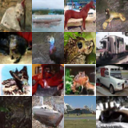
\includegraphics[width=0.9\textwidth]{ddpm_cifar10_grid1.png}
    \caption{google_DDPM}
    \label{fig:cifar10_grid}
\end{figure}

\noindent
之后,我们使用Reproduction一节提到的denoising-diffusion-pytorch包,编写了训练框架,在租用的A800服务器上基于CIFAR-10数据集进行训练,经过15个小时,20000个batch训练(batch size=1024),相当于训练了300多个epoch,得到如下的结果展示:
\begin{figure}[htb]
    \centering
    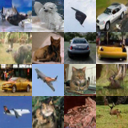
\includegraphics[width=0.9\textwidth]{ddpm_cifar10_grid.png}
    \caption{reproduce_DDPM}
    \label{fig:cifar10_grid}
\end{figure}

\noindent
可以看到,别人的模型就是好!

\noindent
在以上结果的基础上,如前文对应章节所述,我们自己尝试实现了Training代码,仍然使用CIFAR-10数据集,这次因为发现A800太贵了,花了太多钱,所以改在3090上进行训练,经过5个小时,只训练了50个epoch,得到如下的结果展示:
\begin{figure}[htb]
    \centering
    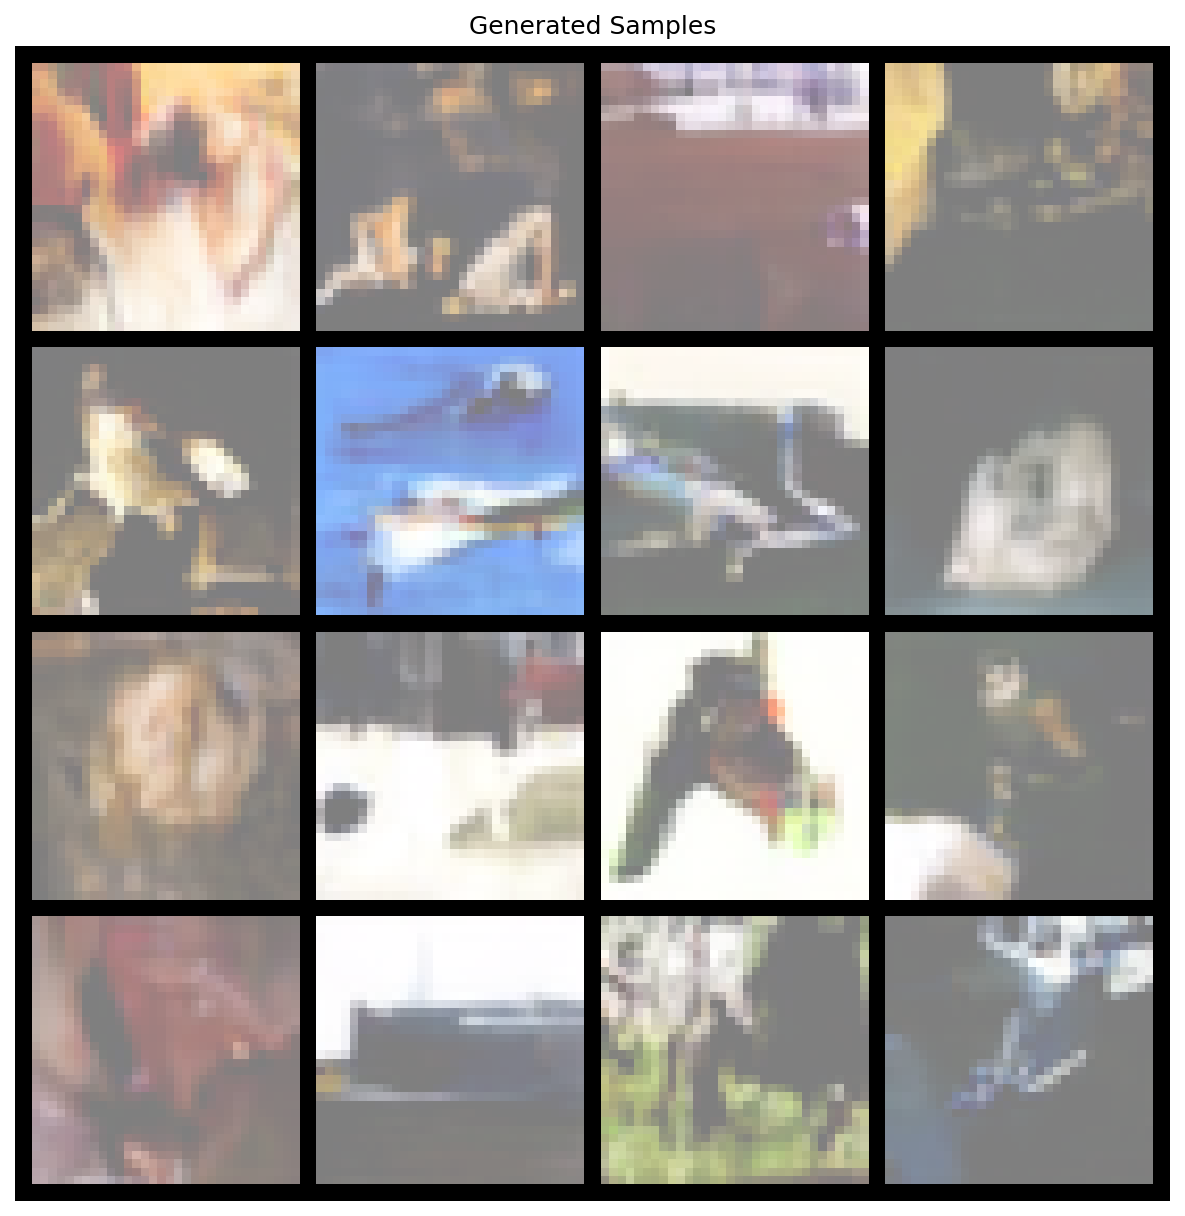
\includegraphics[width=0.9\textwidth]{epoch_50_samples_retrain.png}
    \caption{rewrite_DDPM}
    \label{fig:cifar10_grid}
\end{figure}

\noindent
可以看到,训练效果和别人的模型相比,还是有很大差距的。损失函数如下:
\begin{figure}[htb]
    \centering
    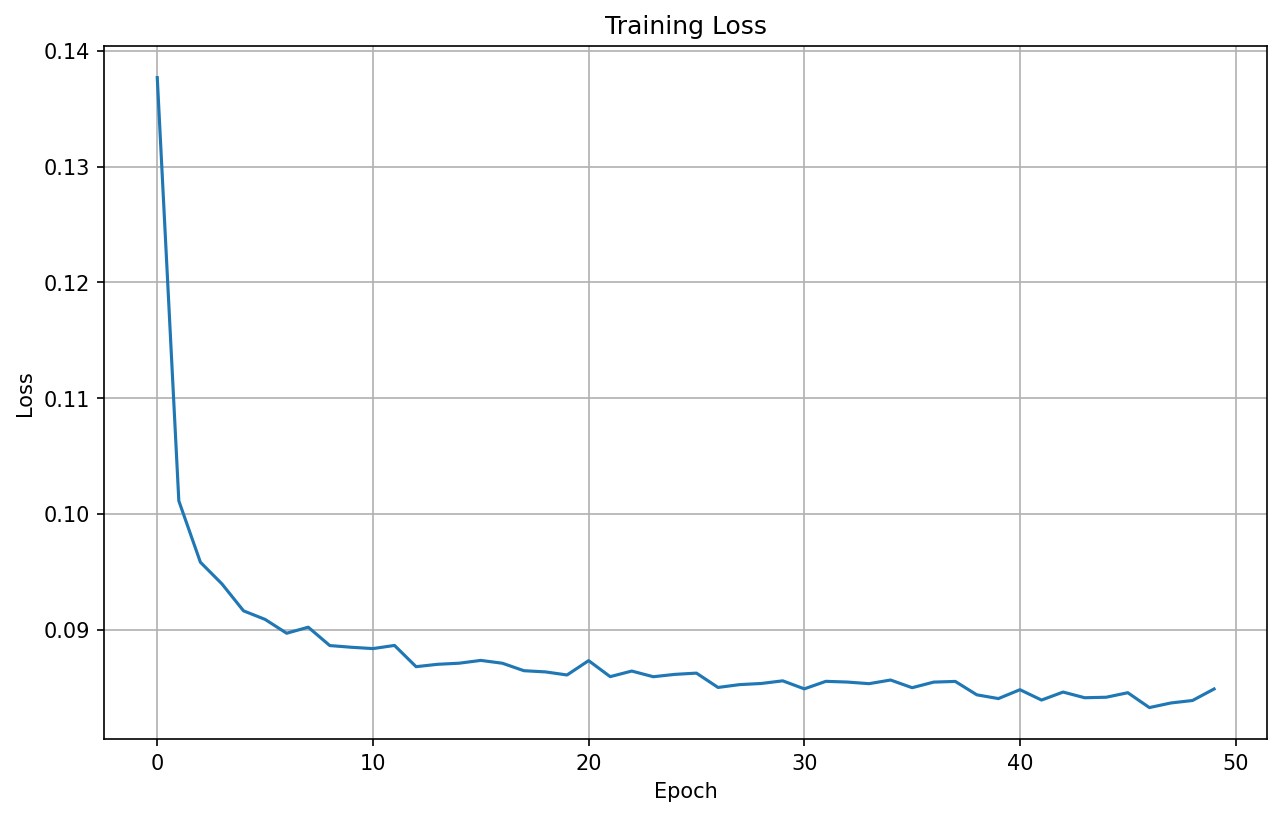
\includegraphics[width=0.9\textwidth]{loss_retrain.png}
    \caption{loss_retrain}
    \label{fig:loss_retrain}
\end{figure}

\noindent
如前所述,由于时间有限,在此基础上,为了在较短时间内能训练较多的轮次,我们对训练代码进行了优化,小幅提高了训练速度,在3090上训练12个小时,训练了250个epoch,得到如下的结果展示:
\begin{figure}[htb]
    \centering
    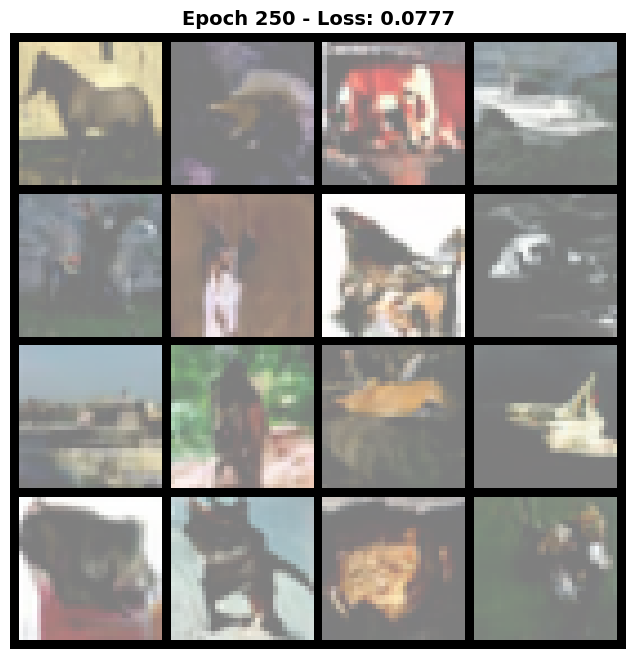
\includegraphics[width=0.9\textwidth]{epoch_250_samples_opt.png}
    \caption{opt_DDPM}
    \label{fig:cifar10_grid}
\end{figure}

\begin{figure}[htb]
    \centering
    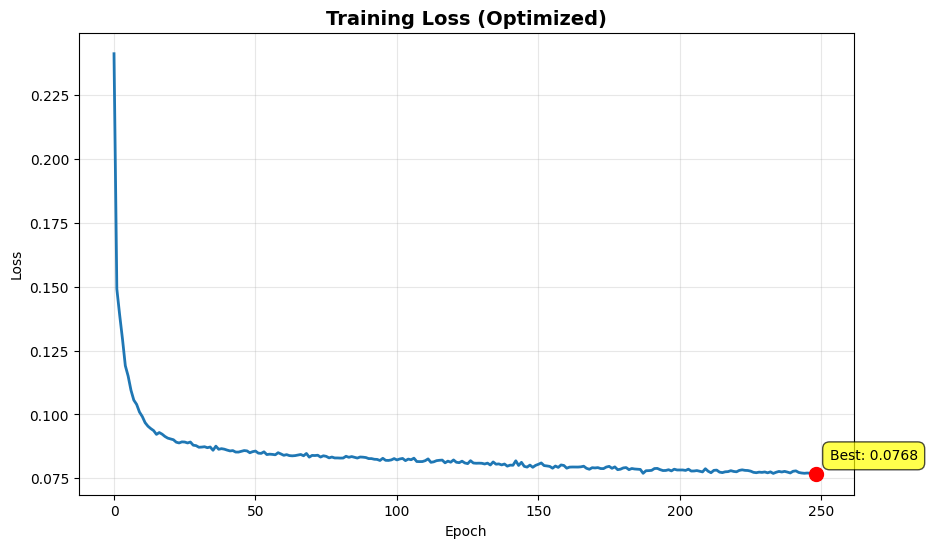
\includegraphics[width=0.9\textwidth]{loss_curve_epoch_250_opt.png}
    \caption{loss_opt}
    \label{fig:loss_retrain}
\end{figure}

\begin{figure}[htb]
    \centering
    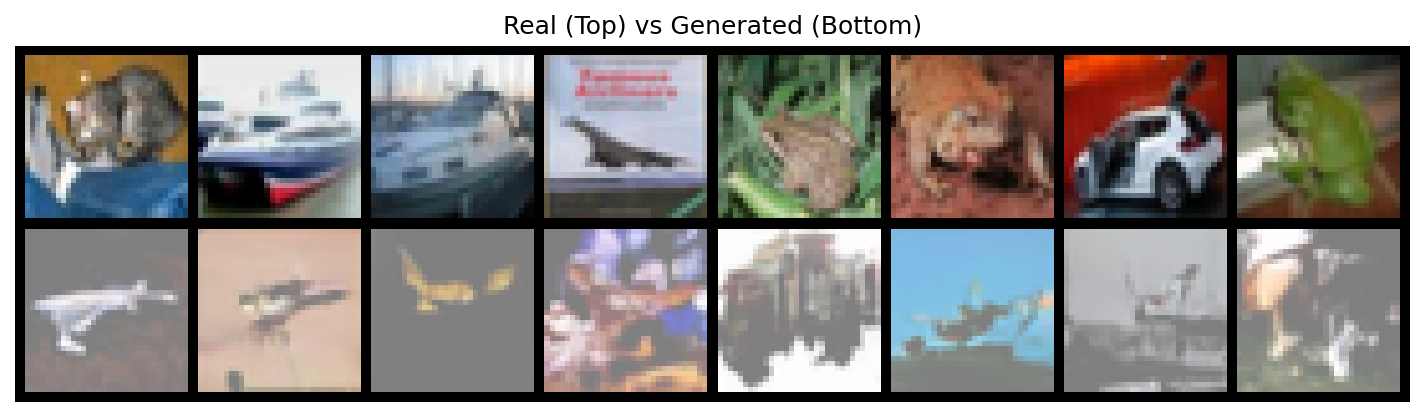
\includegraphics[width=0.9\textwidth]{real_vs_opt.png}
    \caption{real_vs_opt}
    \label{fig:loss_retrain}
\end{figure}

\noindent
可以看到,相比上一次的训练,训练速度明显加快,损失函数下降也更加平缓。生成图片的质量也有一些提升,但和真实图像的差距仍然很大,有很多图片的细节仍然很模糊,比如飞机的螺旋桨,汽车的轮胎等,难以辨认。

\noindent
为更清晰地展现生成结果,我们尝试在分辨率更高的stl10数据集(96*96)上进行训练,由于分辨率很高,训练速度显著降低,条件有限,我们只能使用3090训练12个小时,训练了50个epoch,得到如下的结果展示:
\begin{figure}[htb]
    \centering
    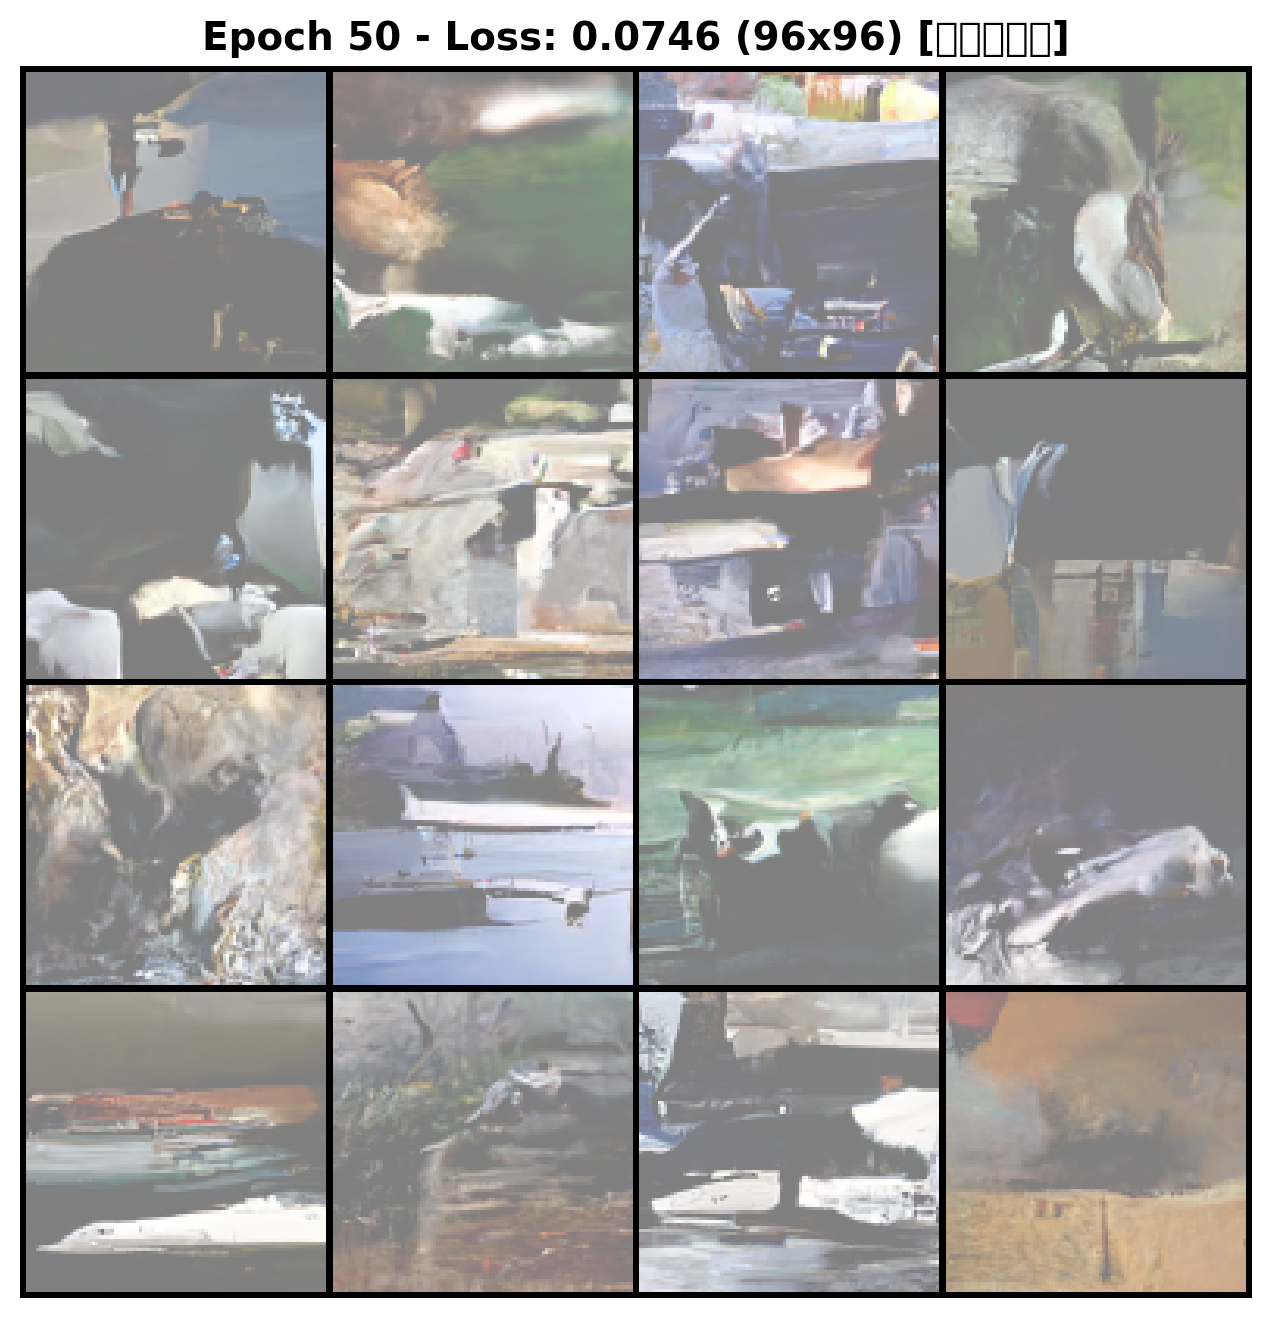
\includegraphics[width=0.9\textwidth]{epoch_50_samples_stl.png}
    \caption{stl10_DDPM}
    \label{fig:cifar10_grid}
\end{figure}

\begin{figure}[htb]
    \centering
    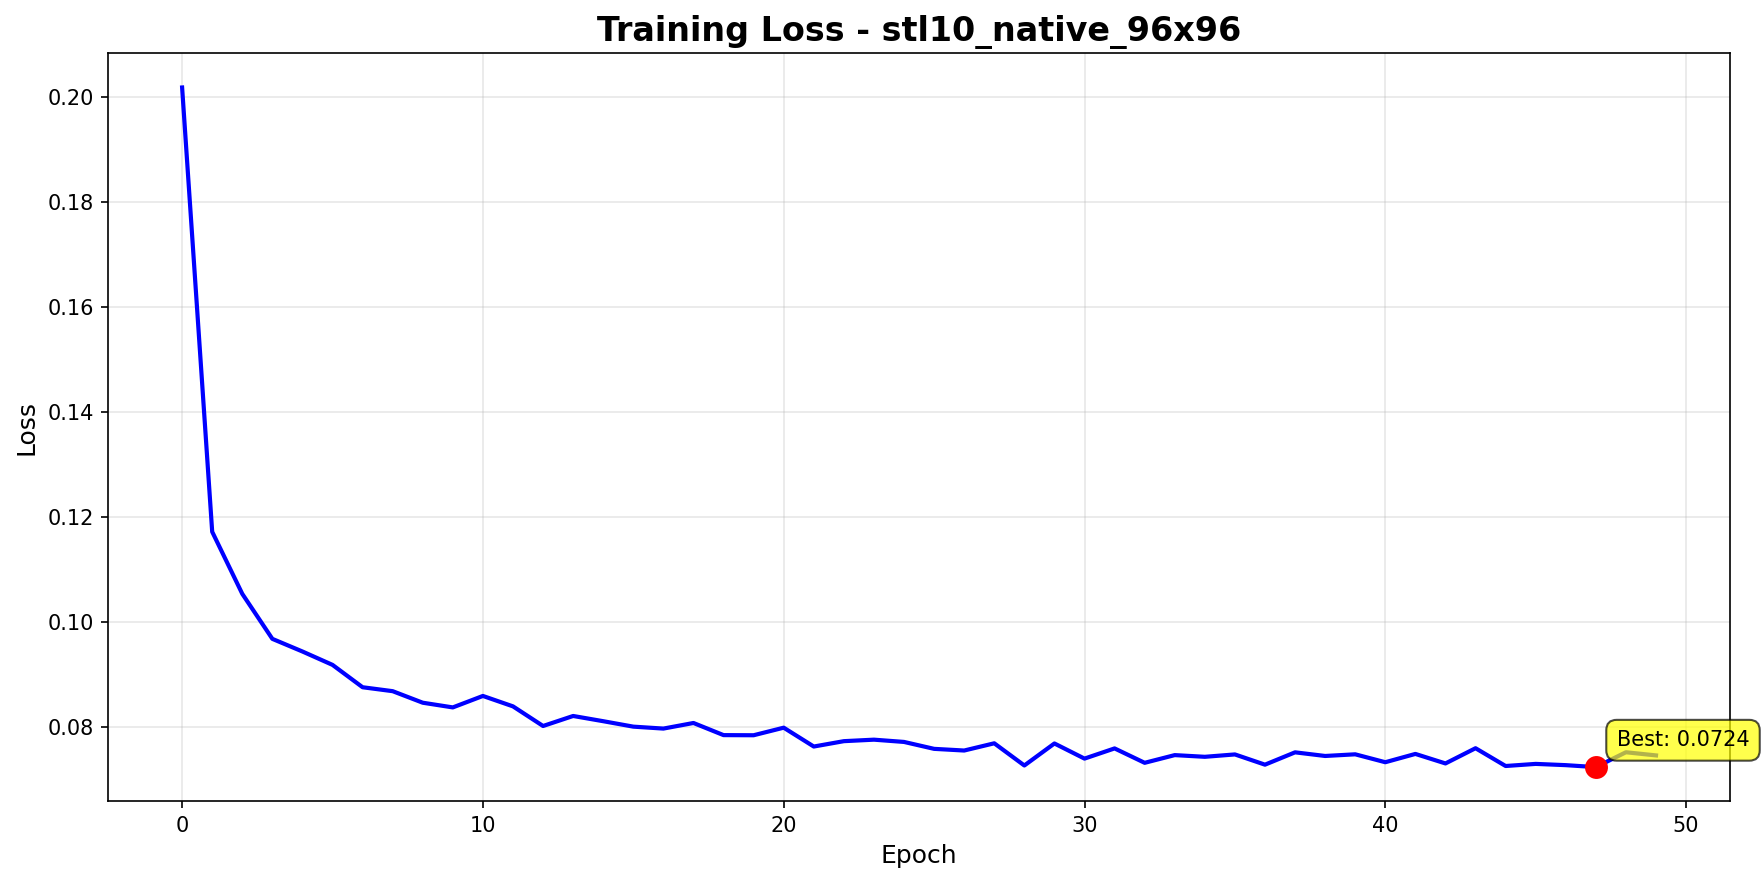
\includegraphics[width=0.9\textwidth]{loss_stl.png}
    \caption{loss_stl}
    \label{fig:loss_retrain}
\end{figure}

\noindent
可以看到,尽管生成的图片几乎看不出是什么,但由于分辨率的增加,各处细节更加清晰,仿佛图片试图在模拟真实世界的某些特征。

\noindent
这时我们注意到,对比参考模型,我们的模型生成的图片明显发灰,几经尝试,无果,遂大改,解决了问题。由于时间有限,没有训练更多轮次,生成图片如下:
\begin{figure}[htb]
    \centering
    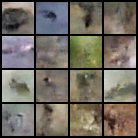
\includegraphics[width=0.9\textwidth]{sample_fix.png}
    \caption{fix_DDPM}
    \label{fig:cifar10_grid}
\end{figure}

\noindent
可以看到,虽然很模糊,但是生成图片不再发灰。

\noindent
接下来,我们尝试对模型的更多细节进行实现,以增加对模型的理解。首先,我们选用了pyTorch的Diffusers库,对模型进行简单的拆解和重新实现,并进行了适当轮次的训练,我们对此模型充满自信,租用A800服务器训练了10个小时,得到了如下的结果展示:
\begin{figure}[htb]
    \centering
    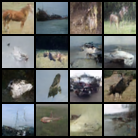
\includegraphics[width=0.9\textwidth]{sample_diffuser.png}
    \caption{diffuser_DDPM}
    \label{fig:cifar10_grid}
\end{figure}

\noindent
可以看到,生成图片质量明显提高,写得好,钱没白花。

\noindent
最后,我们花了大量时间,参考网上的博客文章,使用纯pyTorch从头实现了一个DDPM模型,并进行了训练,在A800上训练6个小时,得到了如下的结果展示:
\begin{figure}[htb]
    \centering
    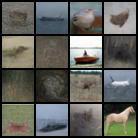
\includegraphics[width=0.9\textwidth]{sample_pyt.png}
    \caption{pyt_inference}
    \label{fig:cifar10_grid}
\end{figure}

\noindent
图片中可以清楚地看到右下角的小马,第一排的小鸟,还有飞机、轮船以及一些其它动物。对比参考模型,可以看到,我们的结果色调更加真实,但是对于和背景颜色比较接近的主体边缘不够清晰。但是总体令人满意。

\section{Conclusion}


\section{References}

    
\end{document}
